
\chapter{Introduction}





\label{chapitre1}
		
		
\includegraphics [width=1 \linewidth, height=0.8\textheight, keepaspectratio] {images/chaptersFigures/intro.png}
		
	
		
    \newpage
    \thispagestyle{plain}

Health has played an important role in human history, helping civilization, behind the curtains to evolve into the society of today\cite{xu2020privacy}. Recently, the healthcare sector has witnessed the development of a wide range of \gls{iot} devices and applications\cite{nasiri2019security}. And a new field has been unlocked: Healthcare information technology (HIT).

\section{Background}
Healthcare information technology (HIT) has been defined as \enquote{the application of information processing involving both computer hardware and software that deals with the storage, retrieval, sharing, and use of healthcare information, data, and knowledge for communication and decision making\cite{brailer2004decade}} where the oil of it is the Medical Informatics as Morris F Collen defines it: \enquote{Medical informatics is the application of computer technology to all fields of medicine-medical care, medical teaching and medical research}; in other words, the medical informatics is the foundation for the understanding and the practice of the up-to-day medicine. Its basic tool is the computer, the subject of studying and the means by which the aspects and achievement in the new knowledge in studying of a man, his health and disease and functioning of the total health activities is performed\cite{masic2013history}.

Medical informatics as a discipline is still young, in particular when you compare it with other medical disciplines. However, within the past decades, societies in general, and medicine and healthcare in particular, have tremendously changed by the adoption of health information technology. This change has significantly impacted the healthcare field as well\cite{haux2010medical}. As a result,  health information technology improves patient’s safety by reducing medication errors, reducing adverse drug reactions, and improving compliance to practice guidelines. There should be no doubt that health information technology is an important tool for improving healthcare quality and safety\cite{alotaibi2017impact}.


\section{Problem \& motivation}
With the progress of health information technology, the healthcare data is increasingly digitized and, like in most other industries, data is growing in Velocity, Volume and Value. According to Statista\cite{HealthcareDataVolume}, the amount of global healthcare data is expected to increase dramatically by the year 2020. Early estimates from 2013 suggest that there were about 153 exabytes of healthcare data generated in that year. However, projections indicate that there could be as much as 2,314 exabytes of new data generated in 2020 (Figure \ref{fig:dataGenerated}).

\begin{figure}[h!]
    \center
    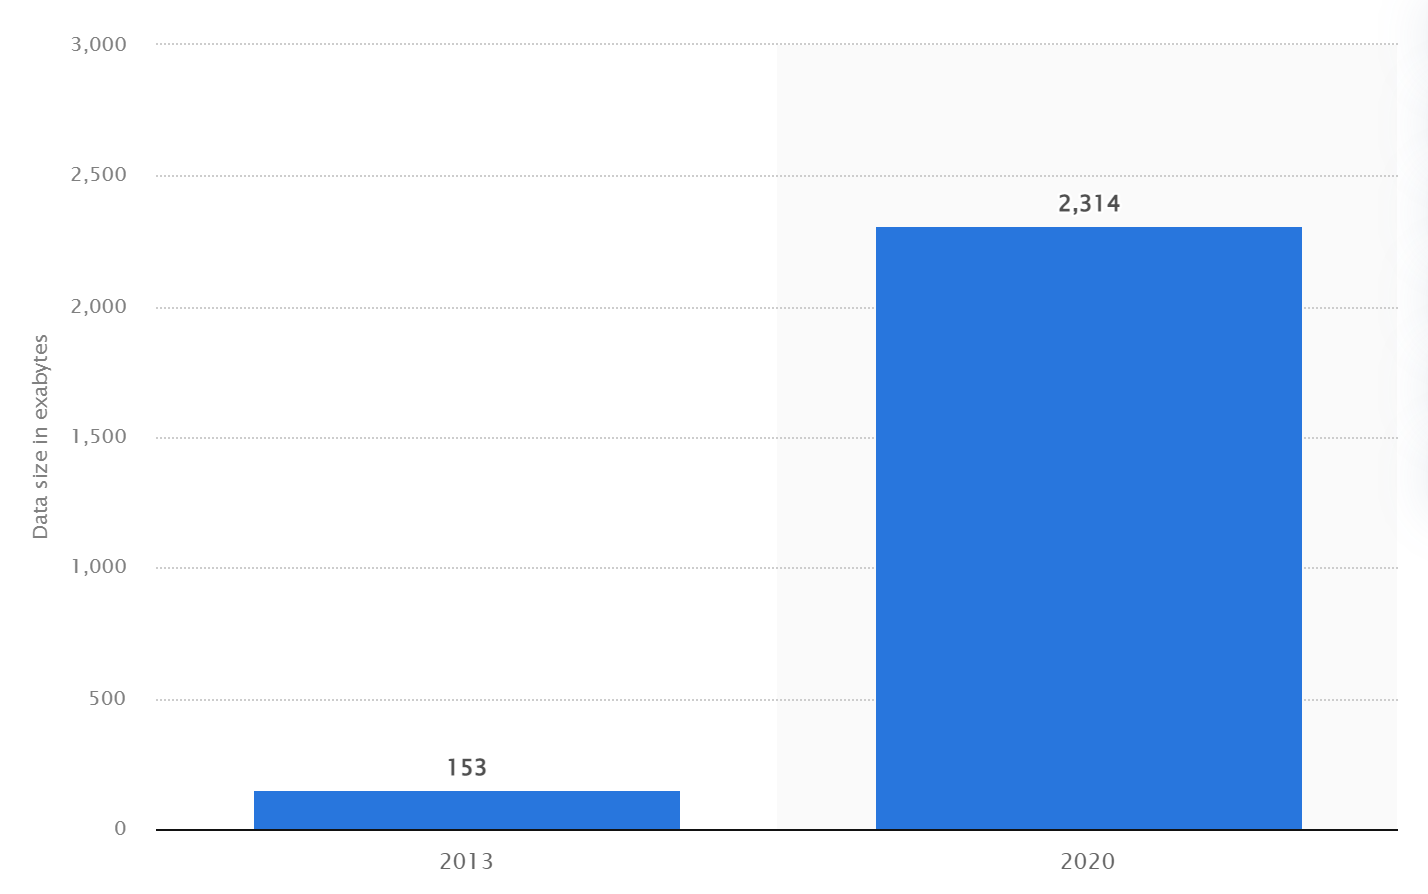
\includegraphics[width=0.75\textwidth]{images/intro/sista.PNG}
    \caption{Total amount of global healthcare data generated in 2013 and a projection for 2020* (in exabytes).}
    \label{fig:dataGenerated}
  \end{figure}

Health Data Management is the practice of making sense of this data and managing it to the benefit of healthcare organizations, practitioners, and ultimately patient wellbeing and health, It enables the integration and analysis of medical data to make patient care more efficient, and extract insights that can improve medical outcomes, while protecting the security and privacy of the data. In the past forty years, medical data began a transition from purely paper-based tracking to digitized information. Even today, many types of medical data have yet to be digitized, or have not yet been integrated into Health Data Management systems. Some of the important challenges facing health data professionals today are\cite{HealthDataManagement}:
\begin{itemize}
  \renewcommand{\labelitemi}{$\bullet$}
    \item \textbf{\textit{Fragmented data:}} medical data can be structured data in spreadsheets or databases, images or video files, digital documents, scanned paper documents, or may be stored in specialized formats such as the DICOM format used for \gls{mri} scans. Data is widely duplicated, collected multiple times and stored in different versions by healthcare providers, public health organizations, insurance bodies, pharmacies, and patients themselves. \textbf{There is no one source of truth for information on patient well being.}
    \item \textbf{\textit{Changes to data:}} medical data constantly changes as do the names, professions, locations and conditions of patients and physicians. Patients undergo numerous tests and are administered many types of treatment over the years, and the treatments and medications themselves evolve over time. New types of medical treatment, such as telehealth models, create new types of data.
    \item \textbf{\textit{Regulations and compliance:}} medical data is sensitive and must adhere to government regulations, such as the USA Health Insurance Portability and Accountability Act (HIPAA). Data discovery challenges and poor data quality make it much more difficult to perform the required audits and meet regulatory requirements and limits the diversity of data healthcare providers can use for the benefit of patients.
  \end{itemize}
  \bigbreak
  In short, these challenges together with the lack of data management systems that provide the right insights to the right actors constitute an obstacle to the development of medical informatics.




\section{Purpose \& delimitations}

The goal of this work is to design a visualization system in medical healthcare that provides personalized dashboards and insights for medical actors.
 
We intend to achieve our goal by designing a visualization system that manages data from different sources, and structures it, then provides a personalized dashboard for each user according to their predefined needs and preferences.
 \newline
 \textbf{First}, we will create a data integration system that takes care of the data management.\newline 
 \textbf{Second}, we will transform the focus data to a structured format.\newline
 \textbf{Third}, we will design a visual presentation after the data processing and formatting in the form of a dashboard web application.

 
\section{Document structure}
This document is presented in 6 chapters, starting with the chapter1: Introduction, in which we present a bit of background of the topic and then delve into formally defining the problem we intend to tackle, followed by a brief description of what lies within and beyond the scope of this work.
 
In Chapter 2: Health sector \& Data, we present the healthcare environment including the principal actors, activities, and the type of data generated from each one. Then we presented the Medical records management and its various electronic types and how important security is to them.
 
In chapter 3: Information Visualization, we present its definition, then we explain the visualization pipeline: how it deals with data, then we move to the data warehouse and its data integration approaches.
 
 Next comes chapter 4: Contribution \& Discussion, we talk about this work's objectives then we go through several related work reviews and, finally, present our proposed work. 
 
 Chapter 5: Implementation, a chapter about the implementation of the system, in which used tools are introduced and results displayed through screenshots and diagrams.
 
Finally, in chapter 6: Conclusion \& Future work, the results and insights gained through the journey of making the proposed solution, few conclusions drawn and perspectives on what could be enhanced moving forward with this project.
